% 02-main/ch2_analysis.tex

\chapter{État de l'art}
\label{chap:analysis}

Ce chapitre dresse un état de l'art des avancées récentes dans la vision par ordinateur, la cartographie du potentiel solaire et l'analyse des toitures. Il examine les différentes méthodes et technologies développées dans ces domaines, en mettant l'accent sur les approches les plus innovantes et leurs applications pratiques.

\localtableofcontents

\newpage

% -----------------------------------------------------------------------------
% -----------------------------------------------------------------------------
\section{Introduction}
\par{L'évaluation du potentiel solaire des toitures est un élément clé de la transition énergétique urbaine. Sa précision dépend directement de la qualité et de la disponibilité des données utilisées, qui peuvent provenir de différentes sources avec des niveaux de détail variables.}

\par{Les méthodologies d'évaluation du potentiel solaire s'appuient principalement sur quatre types de données :}
\begin{enumerate}
    \item Données du cadastre
    \item Modèle tridimensionnel des bâtiments et du territoire
    \item Données géomatiques
    \item Orthophotos
\end{enumerate}

\par{La deuxième partie de ce chapitre va traiter de l'état de l'art en vision par ordinateur.}

\par{Ensuite, une troisième partie sera dédiée aux dataset disponibles.}

\par{Une brève synthèse permettra de conclure et de justifier l'approche utilisée.}

\par{Les notions théoriques nécessaires pour la compréhension de ce chapitre se trouvent dans deux annexes. Le premier traite de  l'énergie solaire et ses applications dans l'annexe ``\nameref{chap:fondamentaux_energie}''. Le deuxième annexe ``\nameref{chap:fondamentaux_ml}'' va permettre d’avoir les bases nécessaires pour comprendre ce qu’est le machine learning, ses
limites et ses applications.}

% -----------------------------------------------------------------------------
% -----------------------------------------------------------------------------
\section{Évaluation du potentiel solaire des toitures}

% -----------------------------------------------------------------------------
\subsection{Analyse du potentiel photovoltaïque des toitures résidentielles en Andalousie}

\subsubsection{Contexte et objectifs}
\par{L'étude menée par \citeauthor{ordonez_analysis_2010} \cite{ordonez_analysis_2010} présente une analyse détaillée du potentiel de production d'énergie photovoltaïque sur les toitures résidentielles en Andalousie (Espagne). Cette région, avec une radiation solaire moyenne de 4,75 kWh/m² par jour et une superficie de 87 597 km², possède le plus fort potentiel solaire d'Europe.}

\subsubsection{Données}
\par{Les données utilisées dans cet article sont :}
\begin{itemize}
    \item Données du cadastre et les surfaces de toiture renseignées lors des autorisations de construire
    \item Orthophotos de google maps
\end{itemize}

\subsubsection{Méthodologie}
\par{La méthodologie repose sur trois volets complémentaires :}
\begin{itemize}
    \item L'analyse statistique des données du cadastre qui répartit les logements en trois types : les maisons individuelles ou jumelées, les maisons en bande, et les immeubles collectifs
    \item L'estimation des surfaces type de toit réellement utilisables pour les panneaux solaires, en prenant en compte tous les obstacles (cheminées, antennes, etc.), les zones d'ombre et les autres contraintes
    \item L'étude de l'ensoleillement moyen de la région et des performances des systèmes photovoltaïques, basée sur les caractéristiques techniques des panneaux disponibles
\end{itemize}

\subsubsection{Résultats principaux}
\par{L'analyse a permis d'identifier les potentiels suivants :}
\begin{itemize}
    \item La surface totale de toiture disponible est de 265,52 km², dont 218,52 km² (82,29\%) sont effectivement utilisables pour des installations photovoltaïques
    \item Le potentiel de production énergétique est estimé à 9,73 GWh/an pour des panneaux IS-170 et 9,38 GWh/an pour des panneaux IS-220
    \item Cette production permettrait de couvrir environ 78,89\% des besoins énergétiques du secteur résidentiel andalou, réduisant la dépendance énergétique extérieure à seulement 21,02\%
\end{itemize}

\subsubsection{Discussion et limites}
\par{Cette recherche démontre qu'il est possible d'estimer le potentiel solaire des toitures à partir de données déjà existantes, sans qu'il soit nécessaire d'investir dans l’acquisition de nouvelles données.}

\par{La méthodologie utilisée, bien que statistiquement solide, présente certaines limites. Notamment, elle s'appuie uniquement sur les données cadastrales issues des autorisations de construire et des enquêtes gouvernementales. Lors de la rédaction de cet article (2010), les auteurs se sont basés sur des données de 2000-2007. Actuellement, ils disposent de données \gls{lidar} \cite{nacional_plan_nodate} qui permettraient une évaluation plus précise et exhaustive du potentiel solaire pour l'Andalousie.}

% -----------------------------------------------------------------------------
\subsection{SolarNet}

\par{}

\subsubsection{Contexte et objectifs}

\subsubsection{Données}

\subsubsection{Méthodologie}

\subsubsection{Résultats principaux}

\subsubsection{Discussion et limites}

% -----------------------------------------------------------------------------
\subsection{Cadastre solaire Genevois}

\par{Il y a une multitude d'article dédiés à l'étude du potentiel solaire, la région de Genève est l'une des régions du monde avec le plus d'articles publiés après Wuhan (Chine) \cite{drozd_evaluating_2025}. \citeauthor{thebault_large-scale_2022} \cite{thebault_large-scale_2022} vont analyser la pertinence de la pose de panneaux solaire \acrshort{pv} au niveau du \gls{grandgeneve}.}

\subsubsection{Contexte et objectifs}
\par{Le premier cadastre solaire de Genève \cite{desthieux_etude_2011} date de 2011. Il est réalisé par hepia, l'EPFL et le Politecnico di Milano, financé par les Services Industriels Genevois et le Service de l'énergie du canton (actuellement l'OCEN). Elle vise à cartographier précisément le potentiel solaire sur les toitures genevoises. Les données utilisées sont :
\begin{itemize}
    \item Données LiDAR de 2009 (4-6 points/m$^2$)
    \item Empreinte au sol des toitures issues du modèle vecteur 3D du bâti sur le canton de 2005
    \item Données météo horaires issues de Meteonorm.
\end{itemize}
La méthodologie utilisée est la suivante :
\begin{itemize}
    \item Construction d'un modèle numérique de surface 2.5D à partir de données LiDAR et d'empreintes au sol des bâtiments
    \item Calcul de l'irradiation solaire horaire sur les toits en tenant compte des ombrages (bâti, végétation, relief), à l'aide d'un outil développé sous Matlab
    \item Production d'indicateurs et de statistiques d'irradiation par toiture dans ArcGIS
\end{itemize}
\par{Le résultat de l'étude est une couche vectorielle qui indique l'irradiation solaire pour la toiture d'un bâtiment. Le temps de calcul est d'environ 2000 h pour une seule machine.}

\par{Une deuxième phase du cadastre est effectuée en 2014 \cite{desthieux_etude_2014} qui permet d'améliorer la modélisation des toitures, le calcul de l'irradiation solaire et de réaliser certains prédimensionnements :
\begin{itemize}
    \item Estimation de production d'électricité
    \item Estimations pour le solaire thermique
    \item Indicateurs économiques
\end{itemize}}
\par{Cette mise à jour positionne le cadastre solaire comme outil d'aide à la décision. Le rendu de l'étude est constitué de plusieurs couches vectorielles. La figure \ref{fig:cadastre_solaire_2014} illustre les informations disponibles.
\begin{figure}[H]
    \centering
    \includegraphics[width=1\linewidth]{02-main//figures/cadastre_solaire_2014.png}
    \caption{Image d'exemple avec une partie des informations disponibles par bâtiment \cite{desthieux_etude_2014}.}
    \label{fig:cadastre_solaire_2014}
\end{figure}

\par{En 2016, le cadastre a été mis à jour \cite{desthieux_solar_2018}. Les principales nouveautés sont :
\begin{itemize}
    \item L'utilisation des données LiDAR de 2013 \cite{sitg_nuages_2013}
    \item L'amélioration des algorithmes de calcul du potentiel solaire
    \item Utilisation d'un cluster (24 machines) pour réaliser les calculs (environ 900h)
\end{itemize}}

\par{Dès 2018, plusieurs mises à jour \cite{desthieux_solar_2018} sont effectuées. Les principales nouveautés sont :
\begin{itemize}
    \item Prise en compte des toitures et des façades des bâtiments pour l'évaluation du potentiel solaire
    \item Amélioration des algorithmes de calcul du modèle de ciel
    \item Réécriture du code Matlab en Java
    \item Utilisation du cloud CTI IceBOUND
    \item Expansion du cadastre solaire au Grand Genève (canton de Genève, district de Nyon, et pôle métropolitain du Genevois Français)
\end{itemize}}

\par{En 2020, l'article \cite{stendardo_gpu-enabled_2020} de \citeauthor{stendardo_gpu-enabled_2020} aborde la question de l'optimisation des calculs pour le cadastre du Grand Genève. Les auteurs proposent l'utilisation des \acrshort{gpu} pour réduire considérablement les temps de traitement. Cette amélioration répond à un défi croissant : chaque nouvelle version du cadastre intègre davantage de données et requiert des calculs plus précis, ce qui allonge inévitablement les temps d'exécution. L'optimisation du code devient donc un aspect fondamental pour la viabilité du projet.
\begin{figure}[H]
    \centering
    \includegraphics[width=1\linewidth]{02-main//figures/cadastre_solaire_gpu.png}
    \caption{Schéma pour le calcul d'une tuile}
    \label{fig:cadastre_solaire_gpu}
\end{figure}
La Figure \ref{fig:cadastre_solaire_gpu} montre comment le traitement a été repensé pour chaque tuile de 3 x 3 km. Les parties du code Java qui pouvaient être massivement parallélisées ont été réécrites en CUDA \cite{nvidia_cuda_nodate}, ce qui permet de tirer parti des \acrshort{gpu} au lieu de s'appuyer uniquement sur les \acrshort{cpu}. Les autres parties critiques du code ont été optimisées en C++ \cite{noauthor_c_2025}. On peut voir sur la Figure \ref{fig:cadastre_solaire_gpu_evolution_temps} que cette approche a permis de réduire considérablement le temps de traitement par tuile.

\begin{figure}[H]
    \centering
    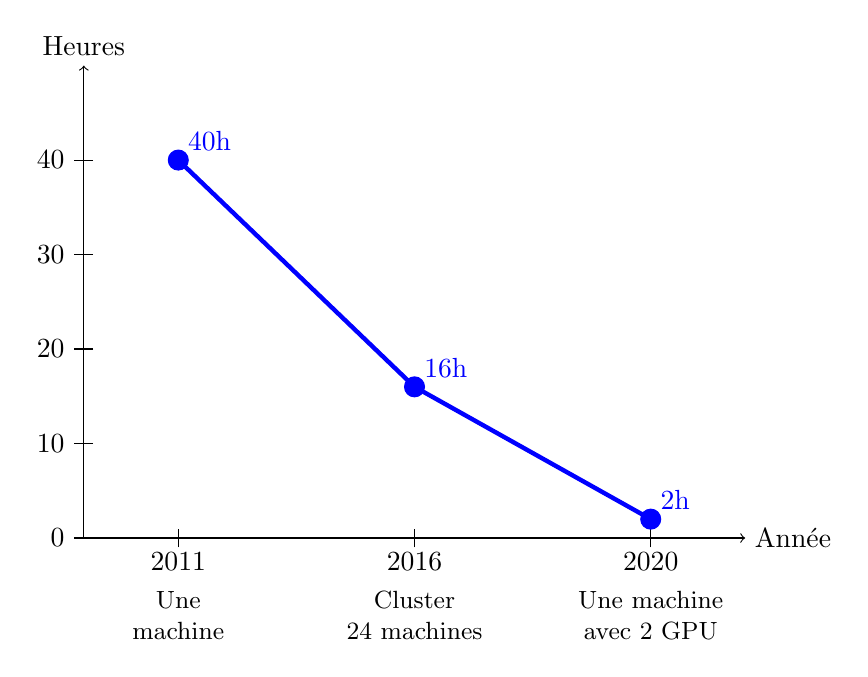
\begin{tikzpicture}[scale=1.2]
        % Axes
        \draw[->] (0,0) -- (7,0) node[right] {Année};
        \draw[->] (0,0) -- (0,5) node[above] {Heures};
        
        % Graduations - en commençant par 1 au lieu de 0
        \foreach \y in {1,2,3,4}
            \draw (0.1,\y) -- (-0.1,\y) node[left] {\y0};
        
        % Ajouter le 0 séparément
        \draw (0.1,0) -- (-0.1,0) node[left] {0};
        
        % Années
        \foreach \x/\year in {1/2011, 3.5/2016, 6/2020}
            \draw (\x,-0.1) -- (\x,0.1) node[below=5pt] {\year};
        
        % Données
        \draw[blue, ultra thick] (1,4) -- (3.5,1.6) -- (6,0.2);
        
        % Points
        \filldraw[blue] (1,4) circle (3pt) node[above right] {40h};
        \filldraw[blue] (3.5,1.6) circle (3pt) node[above right] {16h};
        \filldraw[blue] (6,0.2) circle (3pt) node[above right] {2h};
        
        % Annotations
        \node[align=center, font=\small, below] at (1,0) {\\\\Une\\machine};
        \node[align=center, font=\small, below] at (3.5,0) {\\\\Cluster\\24 machines};
        \node[align=center, font=\small, below] at (6,0) {\\\\Une machine\\avec 2 GPU};
    \end{tikzpicture}
    \caption{Évolution des temps de calcul par tuile pour le cadastre solaire (2011-2020).}
    \label{fig:cadastre_solaire_gpu_evolution_temps}
\end{figure}

\subsubsection{Données}

\subsubsection{Méthodologie}

La méthodologie \cite{desthieux_solar_2018} pour la création du cadastre suit les étapes suivantes :
\begin{itemize}
    \item Collecte des données
    \item Construction du modèle 3D
    \item Calcul des ombrages
    \item Calcul de l'irradiation solaire en chaque point des toits et façades
    \item Calcul des indicateurs et visualisation des résultats
\end{itemize}

La Figure \ref{fig:cadastre_solaire_methodologie} résume ces points.
\begin{figure}[H]
    \centering
    \includegraphics[width=1\linewidth]{02-main//figures/cadastre_solaire_methodologie.png}
    \caption{Méthodologie utilisée pour la création du cadastre solaire \cite{desthieux_solar_2018}}
    \label{fig:cadastre_solaire_methodologie}
\end{figure}

\paragraph{Collecte des données}

\par{La première étape est d'obtenir les données nécessaires ("Raw data" sur la Figure \ref{fig:cadastre_solaire_methodologie}).}
\par{À partir des données LiDAR, on construit deux modèles 3D de la ville : un modèle numérique de surface (DSM) qui représente la surface supérieure des bâtiments et de la végétation, et un modèle numérique de terrain (DTM) qui représente le sol nu sans les bâtiments.}
\par{Les contours et empreintes des toits et bâtiments  sont aussi récupérés à partir de données cadastrales existantes, en 2D et 3D. Ils serviront à délimiter précisément les toits et façades.}

\subsubsection{Résultats principaux}

\subsubsection{Discussion et limites}

% -----------------------------------------------------------------------------
\subsection{ToitSolaire}

\subsubsection{Contexte et objectifs}

\subsubsection{Données}

\subsubsection{Méthodologie}

\subsubsection{Résultats principaux}

\subsubsection{Discussion et limites}
% -----------------------------------------------------------------------------
% -----------------------------------------------------------------------------
\section{Vision par ordinateur}

\par{Ce chapitre va permettre d'explorer l'état de l'art en vision par ordinateur.}

% -----------------------------------------------------------------------------
\subsection{YOLO12}

% -----------------------------------------------------------------------------
\subsection{?}



% -----------------------------------------------------------------------------
% -----------------------------------------------------------------------------
\section{Datasets disponibles}

\par{Quelques datasets de qualité sont disponibles actuellement. Ce chapitre va parcourir certains d'entre eux.}

% -----------------------------------------------------------------------------
\subsection{AIRS}

% -----------------------------------------------------------------------------
\subsection{PASSION}

% -----------------------------------------------------------------------------
\subsection{Roboflow}

% -----------------------------------------------------------------------------
% -----------------------------------------------------------------------------
\section{Solutions commerciales existantes}

\par{Quelques entreprises offrent des solutions pour réaliser un cadastre solaire sur la base de leur données. Dans tous les cas leur méthodologie ou les données utilisées ne sont pas disponible.}

\par{Solargis \cite{solargis_regional_nodate} est spécialisée dans le solaire. Cette entreprise offre diverses solutions pour planifier toutes les phases de chantier, depuis la modélisation d'un site jusqu'au suivi et à l'optimisation des performances des panneaux solaires en phase d'exploitation. Ils offrent aussi la prestation de création d'un cadastre solaire pour une région.}

\par{L'entreprise Picterra \cite{picterra_infrastructure_nodate} offre des solutions pour l'utilisation de machine learning sur des données géomatiques. Entre autres, ils proposent l'estimation du potentiel solaire d'une région. Une autre entreprise suisse, Urbio, \cite{urbio_urbio_nodate} offre aussi des prestations similaires à Picterra mais plus axées sur la planification énergétique.}

\par{Google Projet Sunroof \cite{google_project_nodate} exploite les données de Google pour évaluer le potentiel solaire des différentes régions. Cette plateforme propose également quelques conseils pour l'obtention de subventions. Bien que les données générées soient accessibles au public, Google ne les produit que pour les municipalités et régions qui souscrivent à leurs services. Cette solution est actuellement limitée aux USA.}

% -----------------------------------------------------------------------------
% -----------------------------------------------------------------------------
\section{Synthèse}































\newpage
% -----------------------------------------------------------------------------

This chapter shows example of picture and also serves to populate the different lists: list of figures, list of tables, bibliography, and glossary.

\section{Tables}

This section contains an examples of table: \autoref{tab:esempio}

\begin{table}[H]
	\centering
	\begin{tabular}{ccc}
		\toprule
		name & weight & food \\ 
		\midrule
		mouse	& 10 g	& cheese \\
		cat	& 1 kg	& mice \\
		dog	& 10 kg	& cats \\
		t-rex	& 10 Mg	& dogs \\
		\bottomrule 
	\end{tabular}
	\caption[A floating table]{A floating table.}
	\label{tab:esempio}
\end{table}

\section{Figures}

This section contains examples of figures: \autoref{fig:galleria}, \autoref{fig:lorem}, \autoref{fig:ipsum}, \autoref{fig:dolor}, \autoref{fig:sit}

\begin{figure}[H] 
	\centering 
	\includegraphics[width=0.5\columnwidth]{galleria_stampe} 
	\captionsource{A floating figure}{A floating figure: the lithograph \emph{Galleria di stampe}, of M.~Escher}{\url{http://www.mcescher.com/}}
	\label{fig:galleria} 
\end{figure}

\begin{figure}[H]
	\centering
	\begin{subfigure}[b]{0.45\textwidth}
		\includegraphics[width=\textwidth]{lorem}
		\caption{A gull}
		\label{fig:lorem}
	\end{subfigure}
	~ %add desired spacing between images, e. g. ~, \quad, \qquad, \hfill etc. 
	%(or a blank line to force the subfigure onto a new line)
	\begin{subfigure}[b]{0.45\textwidth}
		\includegraphics[width=\textwidth]{ipsum}
		\caption{A tiger}
		\label{fig:ipsum}
	\end{subfigure}
	~ %add desired spacing between images, e. g. ~, \quad, \qquad, \hfill etc. 
	%(or a blank line to force the subfigure onto a new line)
	\begin{subfigure}[b]{0.45\textwidth}
		\includegraphics[width=\textwidth]{dolor}
		\caption{A mouse}
		\label{fig:dolor}
	\end{subfigure}
	~ %add desired spacing between images, e. g. ~, \quad, \qquad, \hfill etc. 
	%(or a blank line to force the subfigure onto a new line)
	\begin{subfigure}[b]{0.45\textwidth}
		\includegraphics[width=\textwidth]{sit}
		\caption{A mouse}
		\label{fig:sit}
	\end{subfigure}
	\caption{Example subcaption}\label{fig:animals}
\end{figure}


% -----------------------------------------------------------------------------
\section{Code}

\autoref{lst:listing_example} shows an example of Java code rendered with minted.

\begin{listing}
	\javafile{02-main/listings/HelloWorld.java}
	\caption{Example of listing using the minted package}
	\label{lst:listing_example}
\end{listing}

% -----------------------------------------------------------------------------
\section{Other features}

Term (glossaries): \gls{latex}

Acronym (glossaries): \gls{api}

Citation (biblatex): \cite{castello_deep_2019}

% -----------------------------------------------------------------------------
\section{Conclusion}

\blindtext
